\documentclass[11pt]{article}
\usepackage[english,russian]{babel}
\usepackage{url}
\usepackage{graphicx,DCCN2021_ru}

\pagestyle{fancy} 
\fancyhead{} 
\fancyfoot{} 

\usepackage[utf8]{inputenc}
\linespread{1.0}

\usepackage{amsmath}

\makeatletter
\fancyhead[RO]{\small DCCN 2014\\ {№ 1 (39) ' 2014}}
\fancyhead[LO]{\small %А.Б. Первый, В.Г. Второй, и др.
RUSSIAN SCIENTIFIC JOURNAL}

\c@page=1 % Number will be set by publisher.
          % Номер первой страницы, устанавливается издателем.
\makeatother


% Название доклада на русском языке:
\title{ОСОБЕННОСТИ ИЗВЛЕЧЕНИЯ ИНФОРМАЦИИ ИЗ
ТВ-ИЗОБРАЖЕНИЙ ПРИ ОГРАНИЧЕННЫХ ПОТОКАХ
ФОТОНОВ}



\author{Кандидат технических наук В. Н. Бодров
С. А. Казначеев
А. М. Князев}

\begin{document}

% Укажите индекс УДК, соответствующий Вашей работе.
\udk{621.383.724: 681.772.7}

{\let\newpage\relax\maketitle}

\vskip -1.5em


% Аннотация
%%%%%%%%%%%%%%%%%%%%%%%%%%%%%%%%%%%%%%%%%%%%%%%%%%%%%%%%%%%%%%
\begin{abstract}
\textbf{Продемонстрирована возможность извлечения информации из телеви-
зионных изображений при весьма малых потоках оптического излучения, при
которых на каждый элемент (пиксель) фоточувствительной матрицы при-
ходится в среднем один фотон. На базе новейшего типа приёмника изобра-
жения – ПЗС-матрицы с внутренним электронным умножением (Electron
Multiplying CCD, EMCCD), показано, что внутреннее электронное умножение
позволяет существенно повысить отношение сигнал-шум на выходе ПЗС-
приёмника, и приблизиться к теоретическому пределу чувствительности,
ограниченной фотонным шумом.}  
\keywords{ПЗС-матрица, электронное умножение, фотонный шум, ТВ-приёмник, низкая освещён-
ность, отношение сигнал-шум.}
\end{abstract}
%%%%%%%%%%%%%%%%%%%%%%%%%%%%%%%%%%%%%%%%%%%%%%%%%%%%%%%%%%%%%%


\section{Введение}

Развитие приёмных ТВ-устройств сопровождается постоянным повышением
требований к их чувствительности. Результатом прогресса кремниевых матричных ПЗС-приёмников оптического изображения, стало создание фоточувствительных матриц с внутренним электронным умножением – \textit{electron multiplying
CCD (EMCCD)}, способных работать при чрезвычайно низких уровнях освещённости порядка $10^{-4}-10^{-5}$ люкса [1].
Такие матрицы позволяют реализовать субфотонные режимы работы, при которых в
каждый пиксель матрицы в среднем завремя экспозиции попадает менее одного фотона.

Возможность регистрировать с помощью  \textit{EMCCD} одиночные фотоны актуаль-
на в микробиологии, когда исследуемые процессы сопровождаются собственным
свечением биологических объектов, в астрономии, когда требуется реализовать
короткие экспозиции, в физике элементарных частиц, в высокоскоростной спек-
троскопии, при видеонаблюдении в условиях весьма низких освещённостях и ряде
других применений. Получаемые при таких потоках излучения ТВ-изображения обладают рядом особенностей. Они имеют ярко выраженную дискретность, что придаёт им характер близкий к геометрическому шуму, в них практически отсутствуют областиравной яркости, что, как правило, затрудняет непосредственное визуальное восприятие информации и анализ их информационного содержания.

\textbf{Цель работы} теоретически показать возможность регистрации субфотонных изображений и экспериментально продемонстрировать возможность продвижения телевизионных приёмных устройств в область рабочих значений освещённости $10^{-4}$ люкса.

\begin{center}
\textbf{Особенности регистрации субфотонных изображений}
\end{center}

Статистические свойства фотонного шума и процесса регистрации излучения
обычно рассматривают исходя из полуклассической теории фоторегистрации. В
ней рассматриваются только процессы взаимодействия излучения с фоточувствительным материалом в предположении отсутствия пространственно-временных флуктуаций интенсивности излучения.
При этом статистика фоторегистрации соответствуют статистике дискретных
независимых событий, описываемой распределением Пуассона, для которого вероятность наблюдения заданного числа фотоотсчётов во временном интервале от
\textit{t} до \textit{t}+$\tau$ определяется выражением [2]
$$P(N,t,t+\tau)= \frac{(\bar N)^N}{N!} \cdot e^{-N} , (1)$$

где \textit{N} – число фотоотсчётов; $\tau$ – время экспозиции; $\bar N$ – среднее число фотоотсчётов во временном интервале (\textit{t}, \textit{t}+$\tau$). При этом значение отношения сигнал-шум пропорционально квадратному корню из среднего числа регистрируемых фотонов в пикселе матрицы.Анализ зависимостей распределения вероятности показывает, что флуктуации количества зарегистрированных фотонов в пикселе изображения вырождаются в разброс одиночных фотонов по пикселям при малых значениях среднего количества регистрируемых фотонов. Такие изображения называют субфотонными.

В работе проводилось моделирование субфотонных изображений в программе
\textit{MATLAB}. Случайный процесс, представляющий регистрацию фотонов, моделируется с использованием встроенной функции \textit{poissrnd}, генерирующей псевдослучайные целые числа, соответствующие распределению Пуассона, в качестве параметра функции выступает среднее количество фотонов, зарегистрированных в пикселе за время экспозиции – $\bar N$.

На рис. 1, в качестве примера, представлены картины трёх изображений однородного пространственного распределения, полученные в результате моделирования при средних значениях количества фотоэлектронов в пикселе 0.1; 0.01 и 0.001, соответственно.


\includegraphics[width=0.25\linewidth]{1.png}
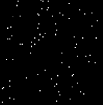
\includegraphics[width=0.255\linewidth]{2.png}

\includegraphics[width=0.267\linewidth]{3.png}

\qquad  \qquad  а)  \qquad  \qquad \qquad  \qquad \quad б)  \qquad  \qquad  \qquad  \qquad  в)

\begin{center}
\textbf{Рис. 1. Примеры изображений, получаемых при различных средних
значениях потоков фотонов}
\end{center}

На рис. 2 даны примеры трёх изображений синусоидальной пространственной
миры. Формат изображений 100х100, период синусоидальной миры численно равен 10 пикселям. Рис. 2. а) иллюстрирует картину, при среднем числе фотонов, приходящихся на пиксель, равном 0.1. На рис 2. б) и 2. в) представлены картины, сформированные потоками фотонов 0.01 и 0.001 фотона на пиксель, соответственно.


\includegraphics[width=0.252\linewidth]{4.png}

\includegraphics[width=0.249\linewidth]{5.png}
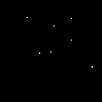
\includegraphics[width=0.25\linewidth]{6.png}

\qquad  \qquad  а)  \qquad  \qquad \qquad  \qquad \quad б)  \qquad  \qquad  \qquad  \qquad  в)

\begin{center}
\textbf{Рис. 2. Изображения синусоидальной миры, реализованные при заданных
величинах фотонного потока в пикселях}
\end{center}

На рис. 2. а) визуально ещё можно наблюдать пространственную периодичность синусоидальной миры. Однако, на рис. 2. б) и 2. в) периодичность визуально
практически незаметна. Поэтому для оценки информационного содержания субфотонных изображений в работе использовался метод корреляционного сопоставления тестового изображения и его субфотонного аналога.

Результаты расчёта коэффициента корреляции в зависимости от величины среднего потока фотонов приведены на рис. 3.

Видно, что при потоках фотонов близких к 0.1 фотона на пиксель, коэффициент корреляции составляет 0.162. При потоках менее 0.01 фотона коэффициент корреляции становится пренебрежимо мал. Таким образом, зависимость на рис.3, указывает на тенденцию снижения информационного содержания изображений
по мере снижения интенсивности фотонного потока.

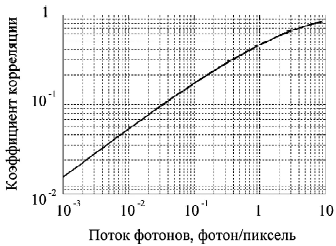
\includegraphics[width=0.8\linewidth]{7.png}

\begin{center}
\textbf{Рис. 3. Зависимость коэффициента корреляции от величины потока фотонов}
\end{center}

Представляет интерес сопоставить результаты моделирования с результатами,
получаемыми при регистрации субфотонных изображений с помощью ПЗС-матриц с внутренним электронным умножением – \textit{electron multiplying CCD (EMCCD)}.
\begin{center}
\textbf{ПЗС-матрицы с внутренним электронным умножением}
\end{center}

Основным фактором, препятствующим получению субфотонных изображений с помощью традиционных ПЗС-устройств, является так называемый шум считывания
[3], который ограничивает возможность реализации требуемого отношения сигнал-шум. Поэтому традиционно основные усилия разработчиков были направлены
на снижение шума считывания. Сегодня наилучшие образцы ПЗС-матриц обладают величиной шума считывания, приближающейся к нескольким шумовым электронам.

Главной особенностью ПЗС-матриц с внутренним электронным умножением
является возможность умножить сигнальный заряд, т. е. увеличить уровень
сигнала ещё до процесса считывания зарядовых пакетов, поэтому шумы считывания в \textit{EMCCD} матрицах отходят на второй план. Это обстоятельство открывает
принципиально новые возможности для повышения отношения сигнал-шум при
весьма низких уровнях освещённости. Такие устройства переводят в практическую плоскость вопрос о возможности регистрации ТВ-камерами субфотонных потоков [4].

В настоящее время известно лишь два производителя ПЗС-матриц с внутренним
электронным умножением – это фирмы \textit{«E2V Technologies»} и \textit{«Texas Instruments»}[5]. Структурная схема фоточувствительной \textit{EMCCD} матрицы приведена на рис.4. Её структура близка к структуре традиционных ПЗС-устройств с кадровым переносом \textit{(frame transfer)}.

Матрица включает в себя секцию экспонирования изображения, секцию хранения электронного изображения и регистр считывания. Отличительной особенностью \textit {EMCCD} устройств является наличие дополнительного регистра – регистра умножения. По структуре регистр умножения близок к регистру считывания, но использует систему электродов с более высоким напряжением тактирующих импульсов. Повышенное напряжение позволяет инициировать лавинный пробой, который приводит к умножению
сигнального заряда. Лавинное умножение происходит при переходе заряда из ячейки в ячейку.

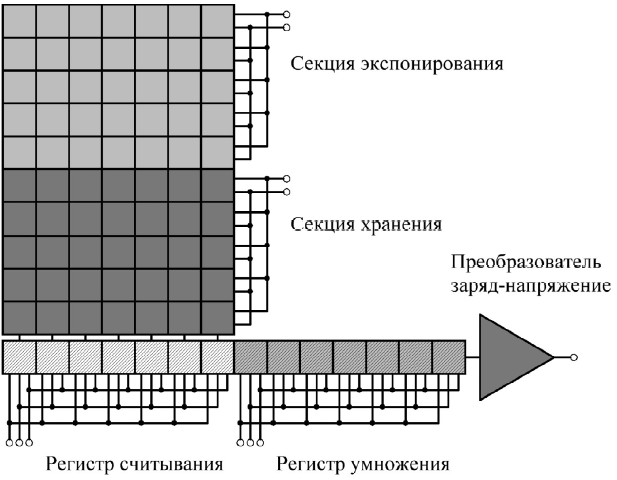
\includegraphics[width=0.8\linewidth]{8.png}
\begin{center}
\textbf{Рис. 4. Структурная схема ПЗС матрицы с внутренним электронным умножением}
\end{center}
Лавинное умножение происходит при переходе заряда из ячейки в ячейку. При каждом таком переходе в результате лавинного умножения исходный заряд увеличивается незначительно, примерно на 1.5-2%, однако после прохождения нескольких сотен
ячеек регистра умножения общий (результирующий) коэффициент умножения может достигать величин порядка ста и выше [6]. Отметим, что при низких значениях коэффициента лавинного умножения процесс электронного умножения является малошумящим, что позволяет увеличивать сигнальный заряд при практически неизменном шуме на выходе матрицы. Таким образом, если пиксель фоточувствительной матрицы регистрирует отдельный фотон, то на вход преобразователя заряд-напряжение поступает сигнальный заряд порядка ста и более
электронов, по сравнению с которым шум считывания становится второстепенным, что и позволяет повысить отношение сигнал-шум.

Важной особенностью \textit{EMCCD} - матриц является использование так называемого обратного освещения матрицы. Обратное освещение матрицы устраняет потери, обусловленные прохождением излучения через электроды, которые характерны для прямой засветки ПЗС структуры, и тем самым приблизить квантовую эффективность \textit{EMCCD} - матриц к теоретическому пределу [7, 8]. Возможность изменения толщины поглощающего слоя при обратном освещении в сочетании с просветляющими покрытиями, позволяет также оптимизировать спектральную кривую квантового выхода. На рис. 5 приведены типичные зависимости спектральной квантовой эффективности \textit {EMCCD} устройств с обратным и прямым освещением.

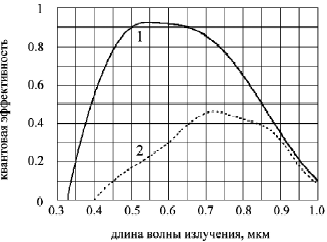
\includegraphics[width=0.8\linewidth]{9.png}
\begin{center}
\textbf{Рис 5. Спектральные зависимости квантовой эффективности для матрицы
с обратным (1) и прямым (2) освещением}
\end{center}

\begin{center}
\textbf{Шумовые свойства EMCCD}
\end{center}

В рассматриваемых устройствах кроме фотонного шума существуют собственные
шумы. Поэтому для определения потенциальных возможностей \textit {EMCCD} устройств
необходим учёт всех составляющих шумовых сигналов. Традиционные ПЗС-матрицы характеризуют отношением сигнал-шум, которое определяется выражением[9]:

$$\frac{\text{сигнал}}{\text{шум}}=\frac{S}{\sqrt{\sigma_R^2+\mathrm{g_T}\cdot\tau+\sigma_{CIC}^2+S}}, (2)$$

где $S$ – среднее значение сигнального заряда; $\mathrm{g_T}$ – скорость процесса термогенерации (электрон на пиксель в секунду); $\tau$– время экспозиции; $\sigma_R$ – шум считывания; $\sigma_{CIC}$ – наведённый шумовой заряд.Для \textit{EMCCD} матриц выражение (2) принимает вид

$$\frac{\text{сигнал}}{\text{шум}}=\frac{S}{\sqrt{\sigma_R^2/M^2+F_{\textit{ш}}^2\cdot(\mathrm{g_T}\cdot\tau+\sigma_{CIC}^2+S)}}, (3)$$

где $M$ – результирующий коэффициент умножения; $F_{\textit{ш}}$ – фактор шума, обусловленный процессом умножения. 

Формула (3) показывает, что высокие значения M позволяют существенно уменьшить влияние шума считывания, т.е. именно того фактора, который принципиально ограничивает чувствительность традиционных ПЗС-устройств.

Шум, обусловленный процессом термогенерации, может быть существенно подавлен при охлаждении \textit{EMCCD} сенсора. Наведённый в нём шумовой заряд, зависящий от количества переносов сигнального заряда из ячейки в ячейку, при тщательном подборе формы управляющих импульсов переноса, составляет незначительную величину менее $10^{-6}$ на каждый перенос [10]. Поэтому при правильном выборе условий работы \textit{EMCCD}-матриц отношение сигнал-шум можно описать выражением

$$\frac{\text{сигнал}}{\text{шум}} = \frac{S}{\sqrt{\sigma_R^2/M^2+F_{\textit{ш}}^2\cdot S}}, (4)$$

При высоких значениях результирующего коэффициента умножения значение
первого слагаемого под корнем в (4) становится соизмеримым со значением составляющей фотонного шума и может стать даже ниже уровня фотонного шума.

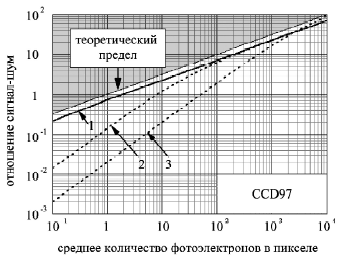
\includegraphics[width=0.8\linewidth]{10.png}
\begin{center}
\textbf{Рис. 6. Отношение сигнал-шум, как функция среднего числа сигнальных
фотоэлектронов в зарядовом пакете. 1 – с умножением при температуре минус 40$^{\text{o}}$С, 2 – при комнатной температуре 20$^{\text{o}}$С и 3 – без умножения}
\end{center}

Зависимости отношения сигнал-шум для \textit{EMCCD} матрицы от величины среднего значения сигнального заряда при различных условия работы, представлены на рис. 6. Для расчёта использованы значения параметров \textit{EMCCD} матрицы типа \textit{CCD97}, характерные для режима работы близкого к телевизионному [11]. Видно, что при охлаждении сенсора до температуры сенсора минус 40$^{\text{o}}$С, отношение сигнал-шум \textit{EMCCD} матриц приближается к теоретическому пределу.

\begin{center}
\textbf{ТВ-устройство на базе \textit{EMCCD} матрицы}
\end{center}

Производство ТВ-устройств на базе \textit{EMCCD} матриц весьма ограничено. В число производителей ТВ-устройств входят ведущие зарубежных фирмы: \textit{«E2V Technologies»}, \textit{«Andor Technology»} (Великобритания) и \textit{«Hamamatsu Photonics»}(Япония). Эти фирмы позиционируют
свою продукцию как устройства для крупных научных центров и лабораторий. Сто
имость их продукции весьма высока. Последнее обстоятельство делает актуальной
задачу разработки и создания собственных устройств, адаптированных для решения конкретных задач.На кафедре электронных приборов НИУ «Московский энергетический институт» было создано ТВ-устройство на базе \textit{EMCCD} - матрицы типа \textit{CCD97} [12], внешний вид которого представлен на рис. 7

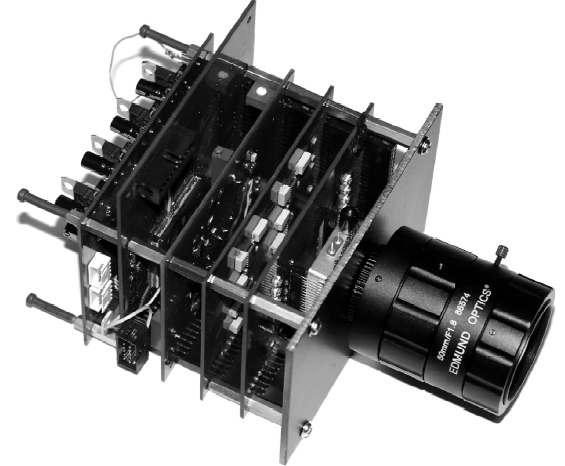
\includegraphics[width=0.8\linewidth]{11.png}
\begin{center}
\textbf{Рис. 7. Внешний вид ТВ-устройства на базе EMCCD матрицы}
\end{center}

Рис. 8 иллюстрирует эффект внутреннего электронного умножения используемой \textit{EMCCD} матрицы. Здесь представлены два изображения, полученные при одинаковой освещённости при различных значениях коэффициента умножения рис. 8 а) – 80 и рис. 8 б) – 3. 

В качестве источника малых фотонных потоков в работе использовалась модель АЧТ типа M-360 фирмы \textit{«Mikron infrared»} (США) при температурах полости от 400 до 600$^{\text{o}}$С. Изображение выходного отверстия АЧТ переносилось в плоскость тест-объекта конденсором с относительным отверстием 1.3 и линейным увеличением равным единице. Тест-объектом служила стандартная штриховая мира. Для получения изображения миры на бесконечности, использовался коллимирующий объектив. Полосно-пропускающий светофильтр типа \textit{Baader} UV-IR Cut использовался для выделения из спектра излучения АЧТ видимого излучения с длинами волн от 420 до 680 нм.

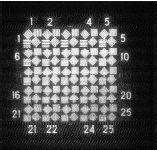
\includegraphics[width=0.249\linewidth]{12.png}
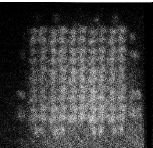
\includegraphics[width=0.25\linewidth]{13.png}

\qquad  \qquad  а  \qquad  \qquad \qquad  \qquad \quad б  \qquad  \qquad  \qquad  \qquad  
\begin{center}
\textbf{Рис. 8. Изображение тест-объекта, полученное с коэффициентом умножения 80 (а) и 3 (б)}
\end{center}

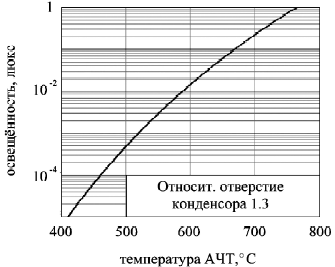
\includegraphics[width=0.8\linewidth]{14.png}
\begin{center}
\textbf{Рис. 9. Зависимость освещённости тест-объекта от температуры излучающей полости АЧТ}
\end{center}

Для сравнения экспериментальных и теоретических результатов использовались значения отношение сигнал-шум, которые рассчитывались по формуле:
$$\frac{\text{сигнал}}{\text{шум}} = \frac{\bar X_\textit{б} - \bar X_\textit{а}}{\sqrt{\sigma^2_X_\textit{а}+\sigma^2_X_\textit{б}}} , (5)$$

Здесь $X$ – среднее значение сигнала; $\sigma_X$ – среднеквадратичное отклонение. Здесь индекс а) относится к закрытым от освещения – опорным пикселям, а индекс б) относится к центральной (рабочей) области кадра при равномерном однородном освещении. На рис. 10 представлена теоретическая зависимость отношения сигнал-шум. Здесь же нанесены полученные экспериментальные значения, полученные притом же значении коэффициенте умножения, равном 80. Видно, что внутреннее электронное умножение является эффективным средством, обеспечивающим работу ТВ-устройств в условиях малой освещённости $10^{-4}$ – $10^{-2}$ люкса.

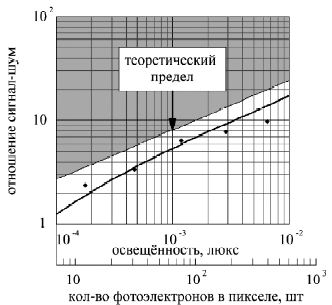
\includegraphics[width=0.8\linewidth]{15.png}
\begin{center}
\textbf{Рис. 10. Теоретическая зависимость и экспериментальные значения отношения сигнал-шум при результирующем коэффициенте умножения M=80}
\end{center}

\begin{center}
\textbf{Выводы}
\end{center}

Рассмотрены особенности формирования изображений потоками излучения,
составляющими единицы фотонов на элемент изображения. Проведено моделирование субфотонных изображений и корреляционное сопоставление моделируемых изображений с исходными образами. Показана возможность извлечения информационного содержания изображений даже при потоках менее одного фотона на элемент изображения.

Рассмотрены особенности фоточувствительных ПЗС матриц с внутренним
электронным умножением (\textit{EMCCD}), ориентированных на получение субфотонных ТВ-изображений. Для конкретного типа \textit{EMCCD} сенсора проведен расчёт реализуемых значений отношения сигнал-шум при регистрации изображений. 

Разработано и создано ТВ-устройство на базе \textit{EMCCD} сенсора, позволившее продемонстрировать эффективность использования внутреннего электронного умножения сигнала для повышения отношения сигнал-шум. Полученные результаты показывают возможности и перспективы продвижения ТВ-устройств в область сверхнизких значений освещённости и получения малофотонных (субфотонных) ТВ-изображений.

\begin{thebibliography}{99}
\bibitem{bib1}  %% citation code
\url{http://www.andor.com}

\bibitem{bib2} Гудмен Дж. Статистическая оптика / пер. с англ. – М.: Мир, 1988. – 528 с

\bibitem{bib3} Janesick James R. Scientific charge-coupled device, The society of Photo-Optical
Instrumentation Engineering, Bellingham, 2001. – 906 p.

\bibitem{bib4} Бодров В. Н., Казначеев С. А., Обидин Г. И. Малофотонные телевизионные изоб-
ражения, их реализация и проблемы // Современное телевидение и радиоэлектроника.
Тр. 19-й МНТК, Москва, Россия, 15-16 марта 2011 г. – М.: ФГУП МКБ «Электрон»,
2011. – 356 с.
    
\bibitem{bib5} Donal J. Denvir, Emer Conroy Andor Technology Ltd. UK Electron Multiplying CCD Technology: The new ICCD. – \url{http://www.emccd.com/downloads/pdfs/EMCCD%20The%20New%20ICCD.pdf}

\bibitem{bib6} Donal J. Denvir. Emer Conroy Electron multiplying CCDs, Published: 19 March 2003; 14 pages; 29 papers // Proc. SPIE. – Vol. 4877.
    
\bibitem{bib7} Paul R Jorden, Mark Downing, Andrew Harris. Improving the red wavelength sensitivity of CCDs, Published: 2 July 2010; 11 pages; 68 papers // Proc. SPIE. – Vol. 7742
    
\bibitem{bib8} George M. Williams, Jr., Alice L. Reinheimer, C. Bruce Johnson. Back-illuminated and electron-bombarded CCD low light level imaging system performance Published: 8 September 1995; 16 pages; 32 papers // Proc. SPIE. – Vol. 2551.

\bibitem{bib9} E2V Technologies Low-Light Technical Note 2 The Use of Multiplication Gain in
L3VisionTM Electron Multiplying CCD Sensors A1A-Low-Light Technical Note 2 Issue 4, July 2003. – \url{http://www.e2v.com/e2v/assets/File/documents/imaging-space-and-scientificsensors/Papers/low_light_technical_note_2.pdf}

\bibitem{bib10} Wen W. Zhang, Qian Chen, Bei B. Zhou and Wei J. He Signal-to-Noise Ratio Improvement of EMCCD Cameras World Academy of Science, Engineering and Technology 41 2010. – \url{http://www.waset.org/journals/waset/v41/v41-208.pdf}

\bibitem{bib11} CCD97-00 Back Illuminated 2-Phase IMO Series Electron Multiplying CCD Sensor. \url{http://www.e2v.com/assets/media/files/documents/imaging-space-and-scientific-sensors/CCD97_BI.pdf}

\bibitem{bib12} Казначеев С. А. / рук. к. т. н., проф. В. Н. Бодров. Реализация ТВ-камеры на базе фоточувствительной EMCCD-матрицы // Радиоэлектроника, электротехника и энергетика: Тр XIX МНТК студентов и аспирантов. – М.: МЭИ, 2013.

\end{thebibliography}

\end{document}